\newpage

\section{Pesquisa Inicial}\label{app_b:inicial}
% Texto da primeira secao do primeiro anexo

\begin{figura}[ht]
	\centering
	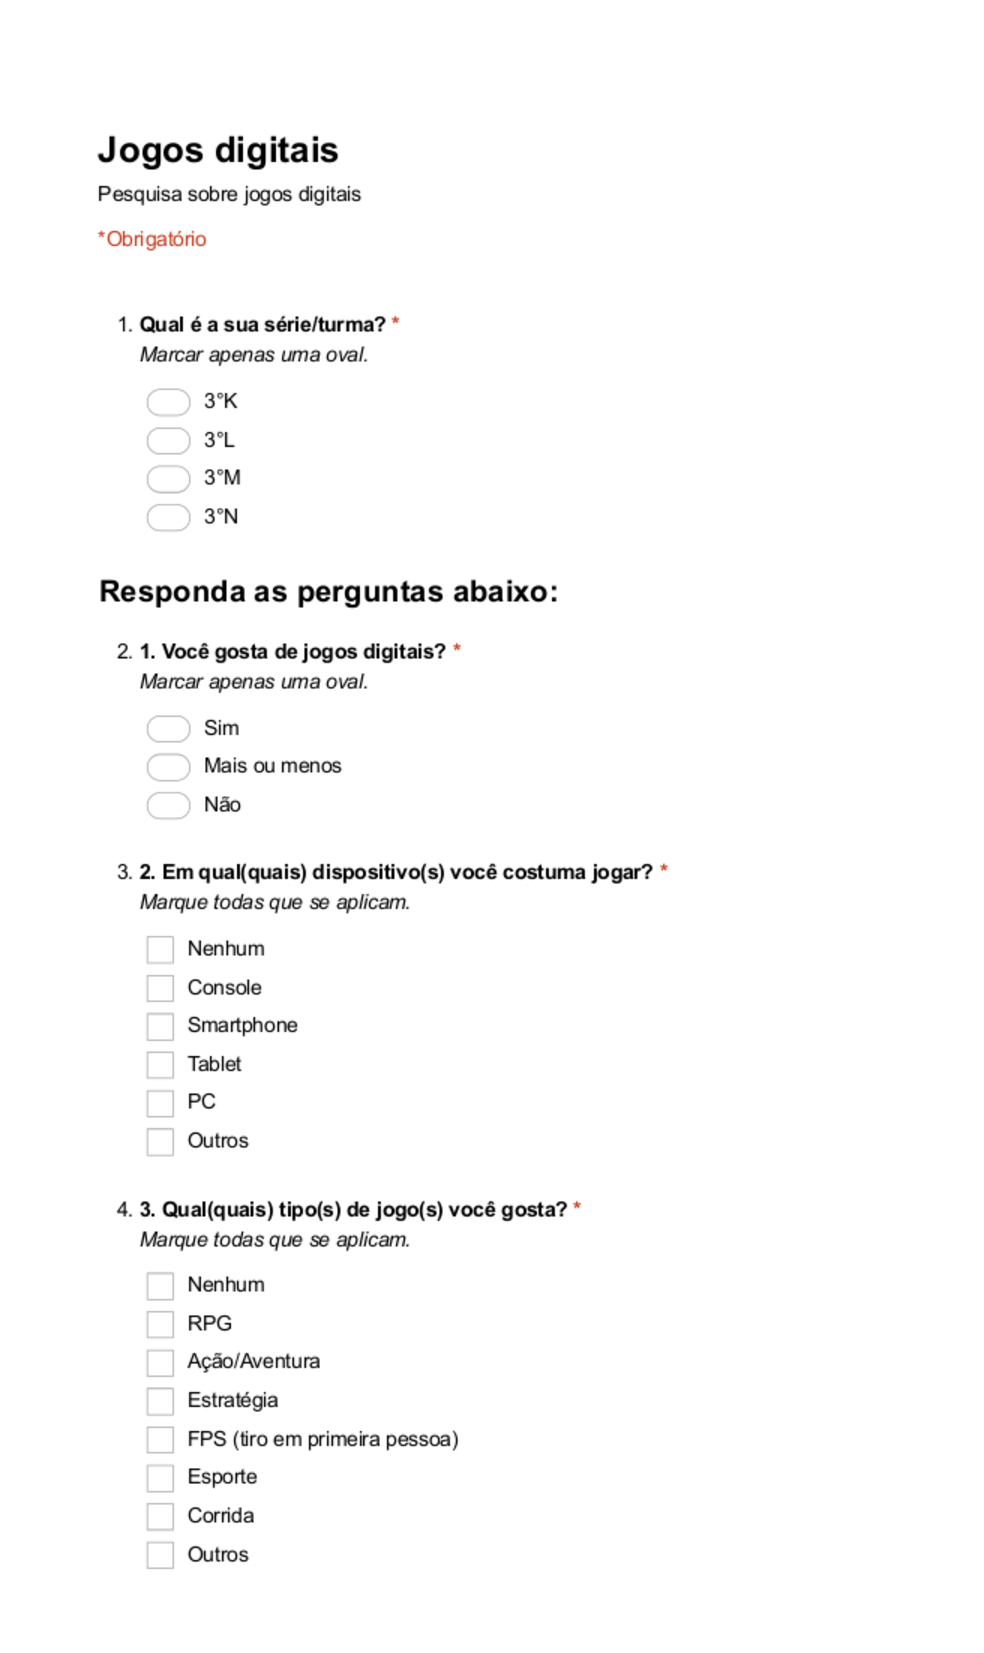
\includegraphics[width=0.69 \textwidth]{ApeB/Img_pesq_ini/pi_part1}
	\caption{Pesquisa inicial: parte 1}
	\label{fig:pf_perg_16}
\end{figura}

\newpage

\begin{figura}[ht]
	\centering
	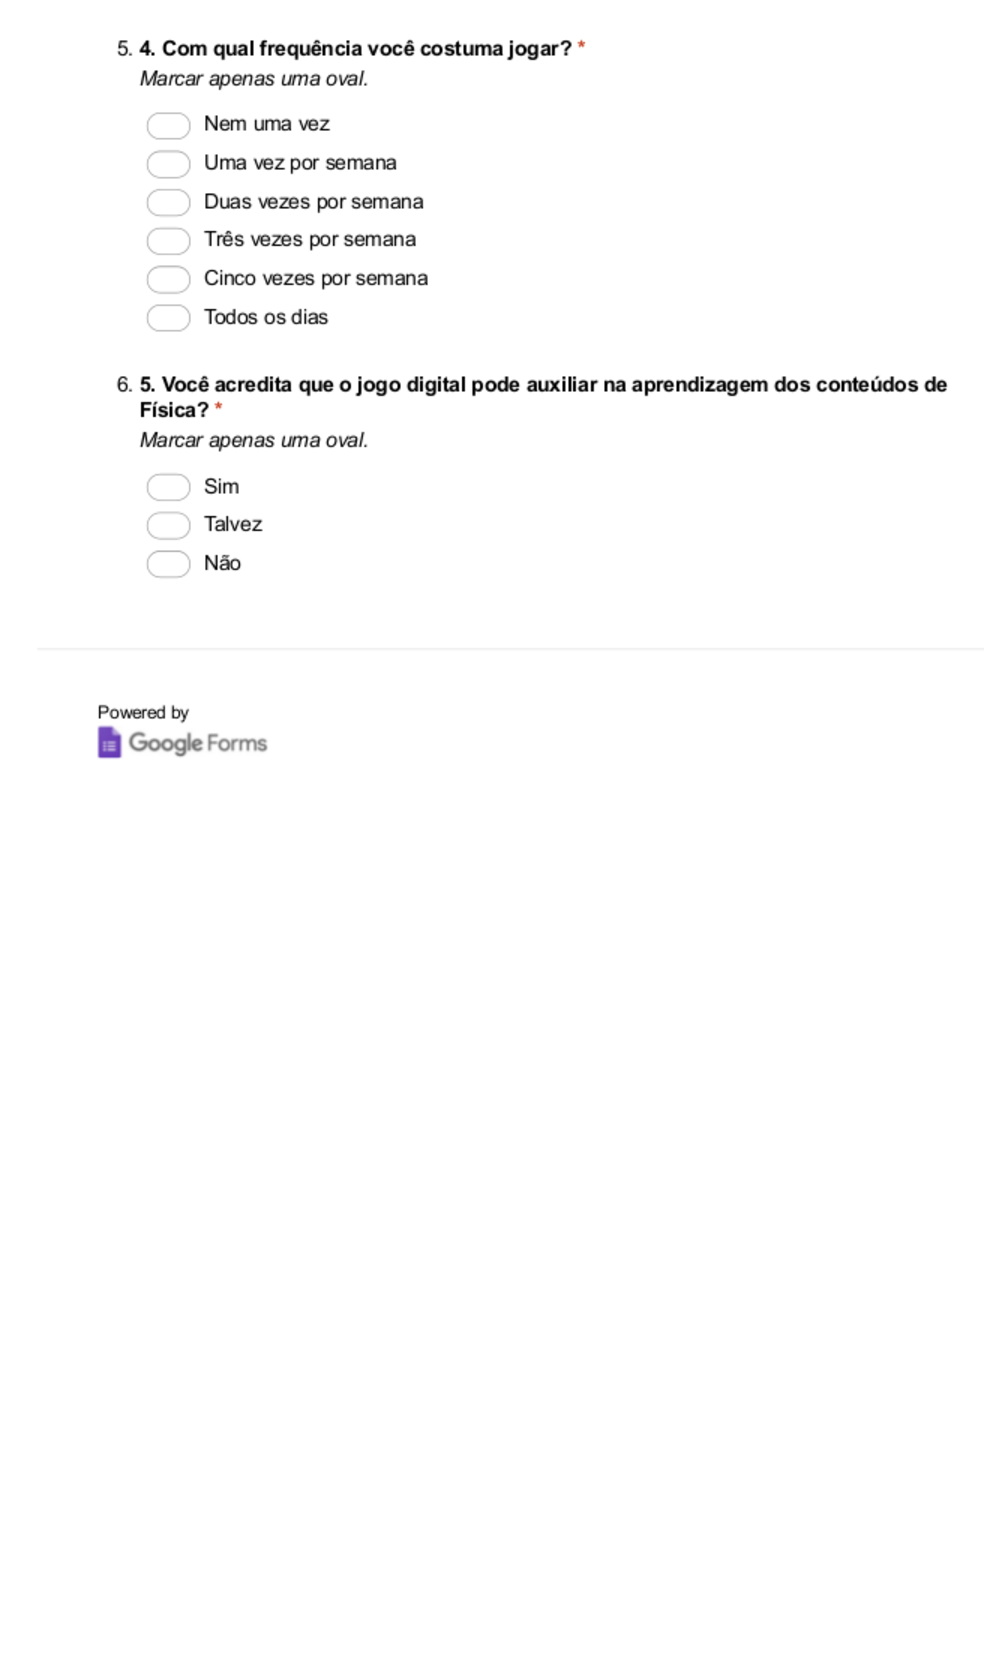
\includegraphics[width=0.69 \textwidth]{ApeB/Img_pesq_ini/pi_part2}
	\caption{Pesquisa inicial: parte 2}
	\label{fig:pf_perg_16}
\end{figura}

\newpage

\section{Testes}\label{app_b:teste}

\begin{figura}[h]
	\centering
	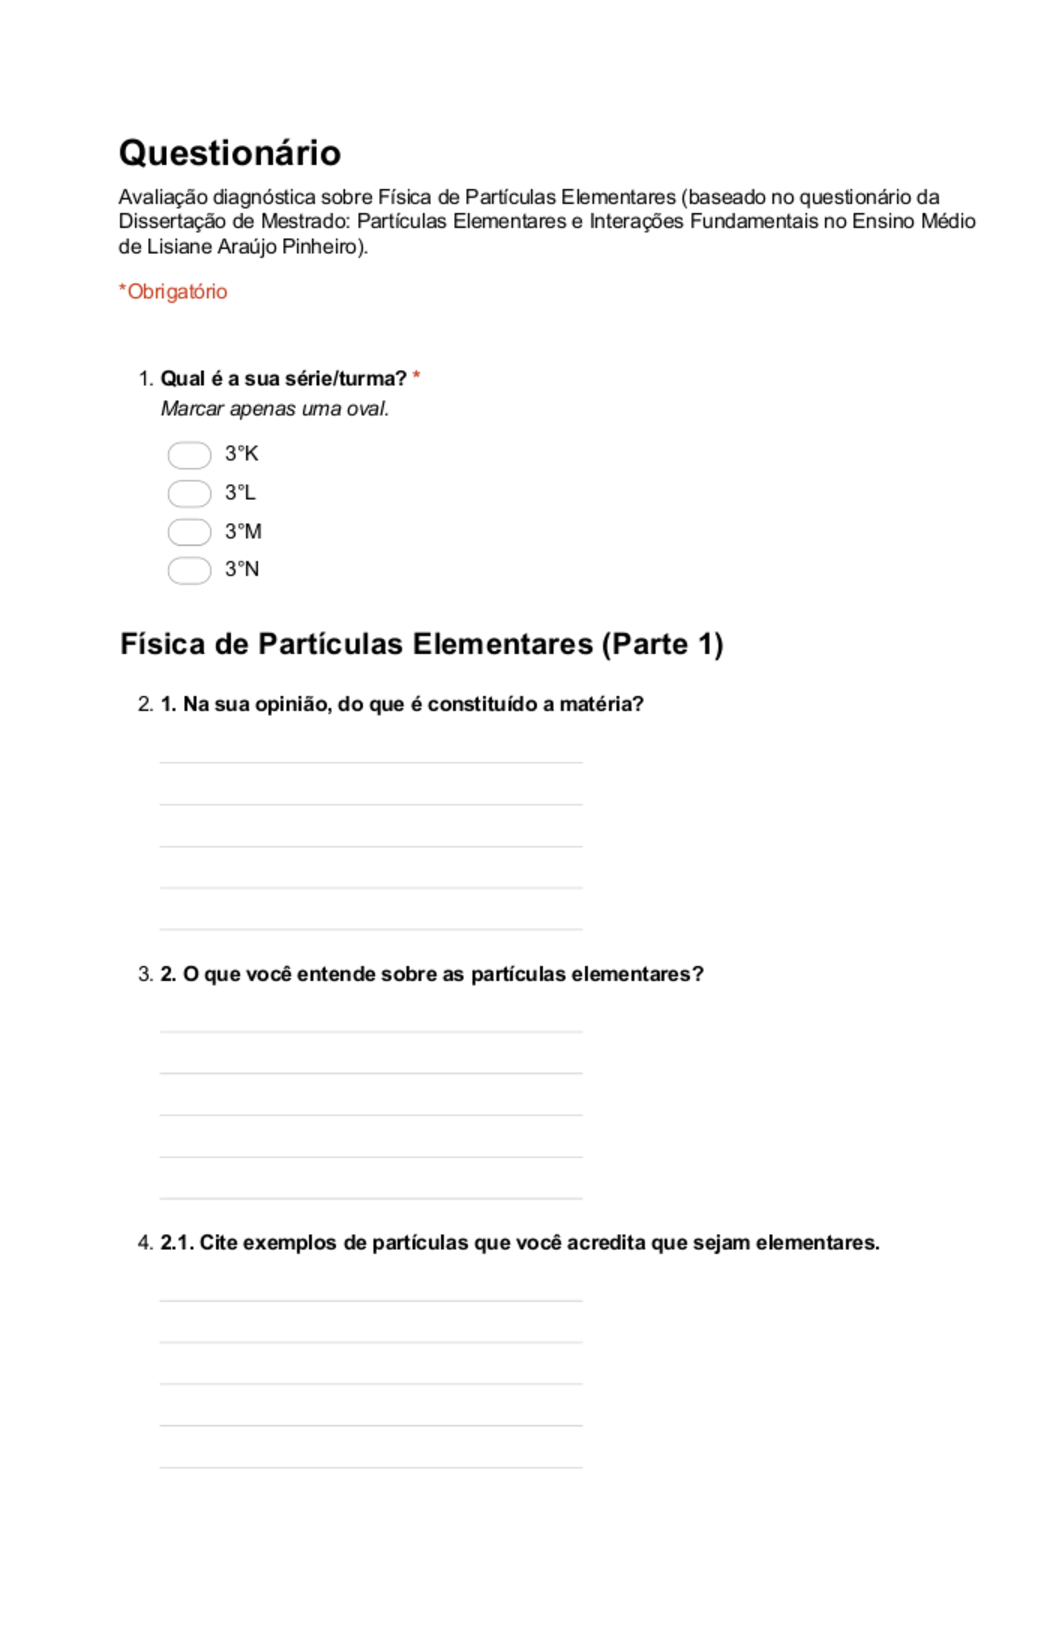
\includegraphics[width=0.70 \textwidth]{ApeB/Img_test/teste_part1}
	\caption{Teste: parte 1}
	\label{fig:pf_perg_16}
\end{figura}

\newpage

\begin{figura}[ht]
	\centering
	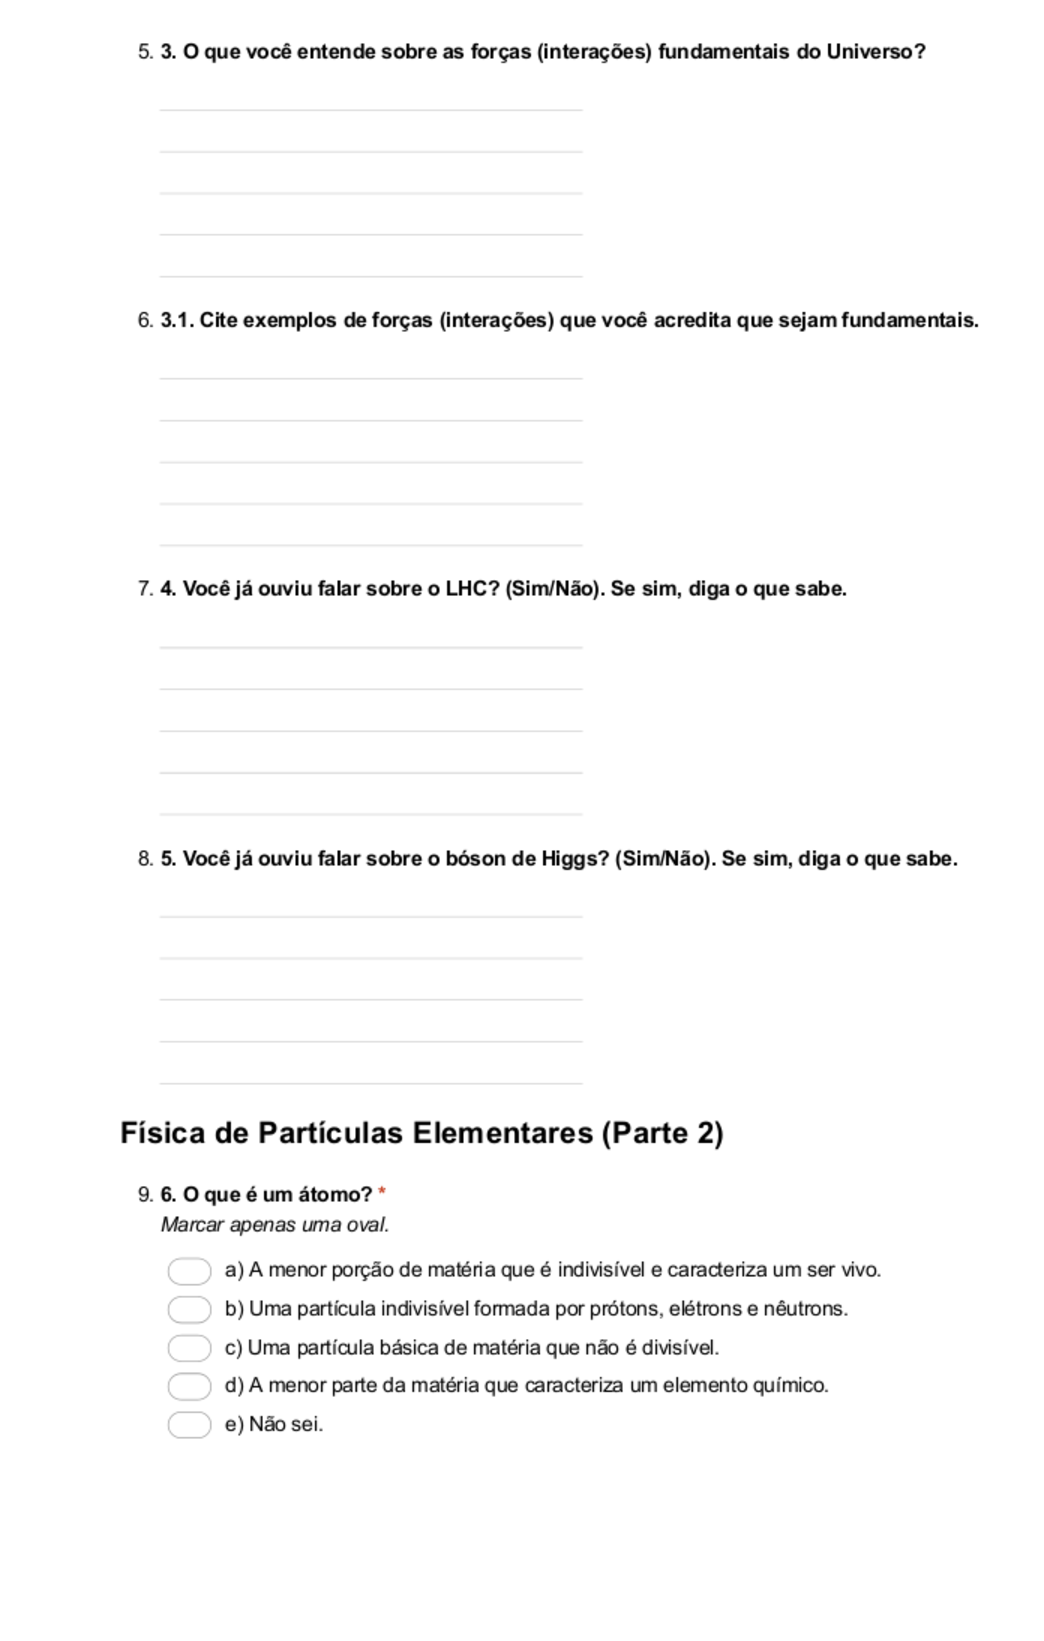
\includegraphics[width=0.70 \textwidth]{ApeB/Img_test/teste_part2}
	\caption{Teste: parte 2}
	\label{fig:pf_perg_16}
\end{figura}

\newpage

\begin{figura}[ht]
	\centering
	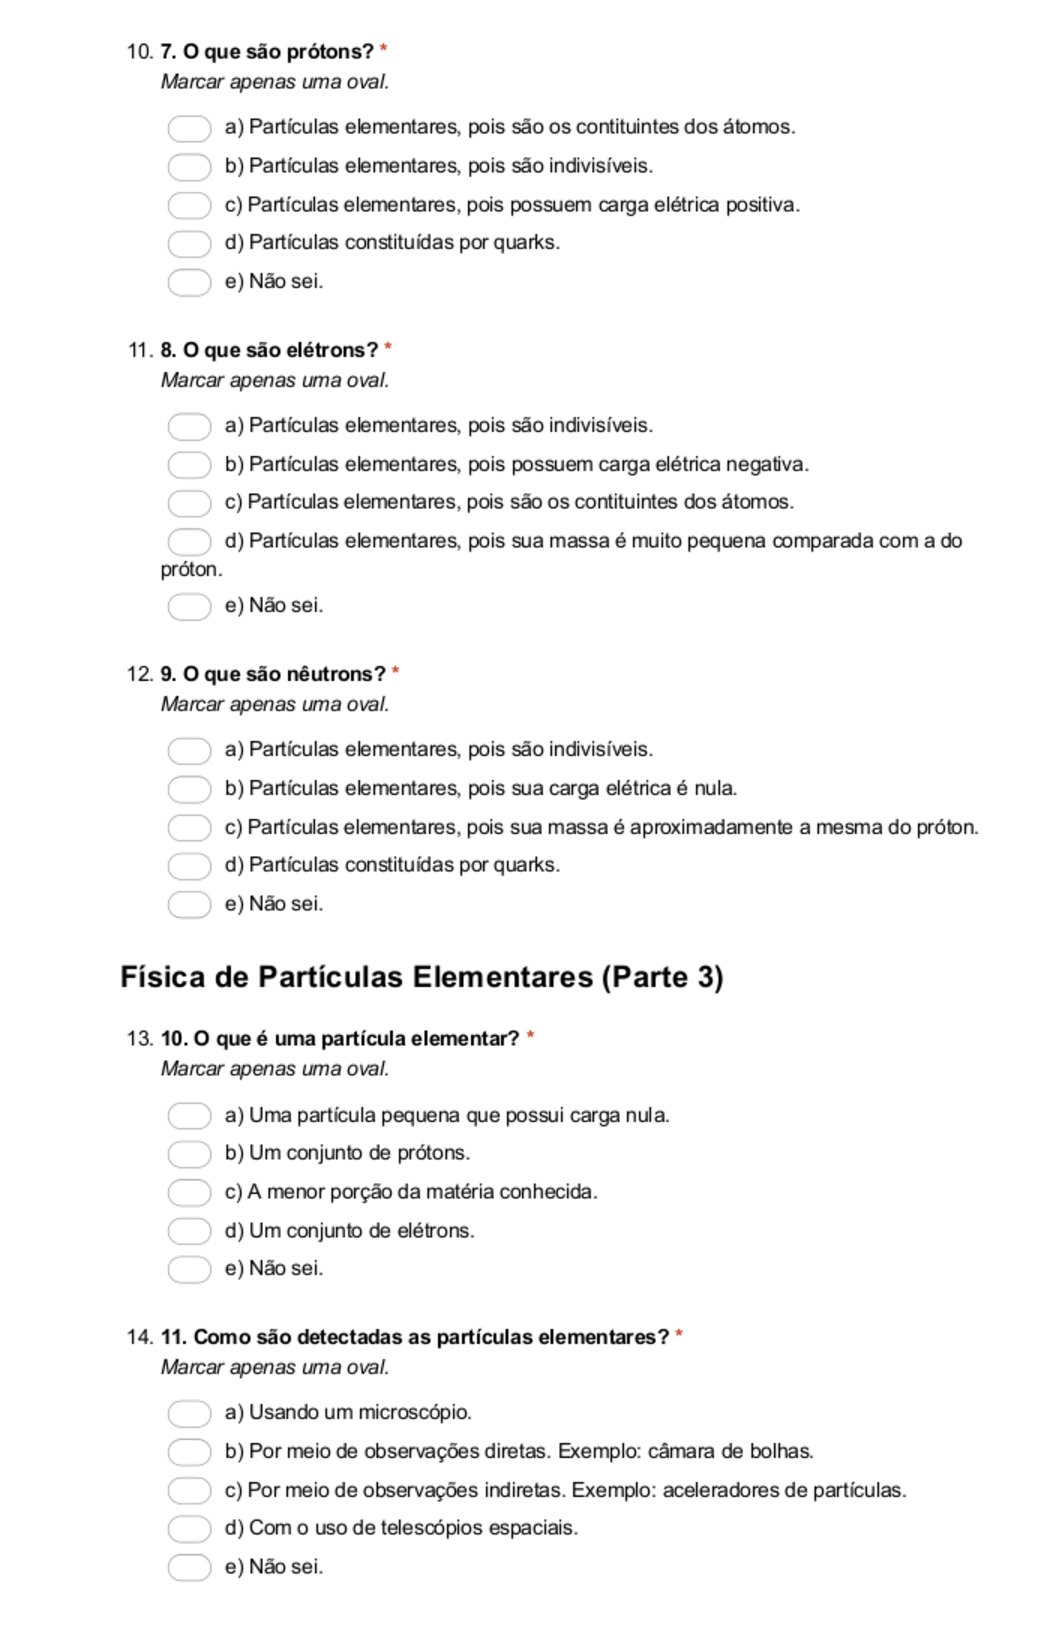
\includegraphics[width=0.70 \textwidth]{ApeB/Img_test/teste_part3}
	\caption{Teste: parte 3}
	\label{fig:pf_perg_16}
\end{figura}

\newpage

\begin{figura}[ht]
	\centering
	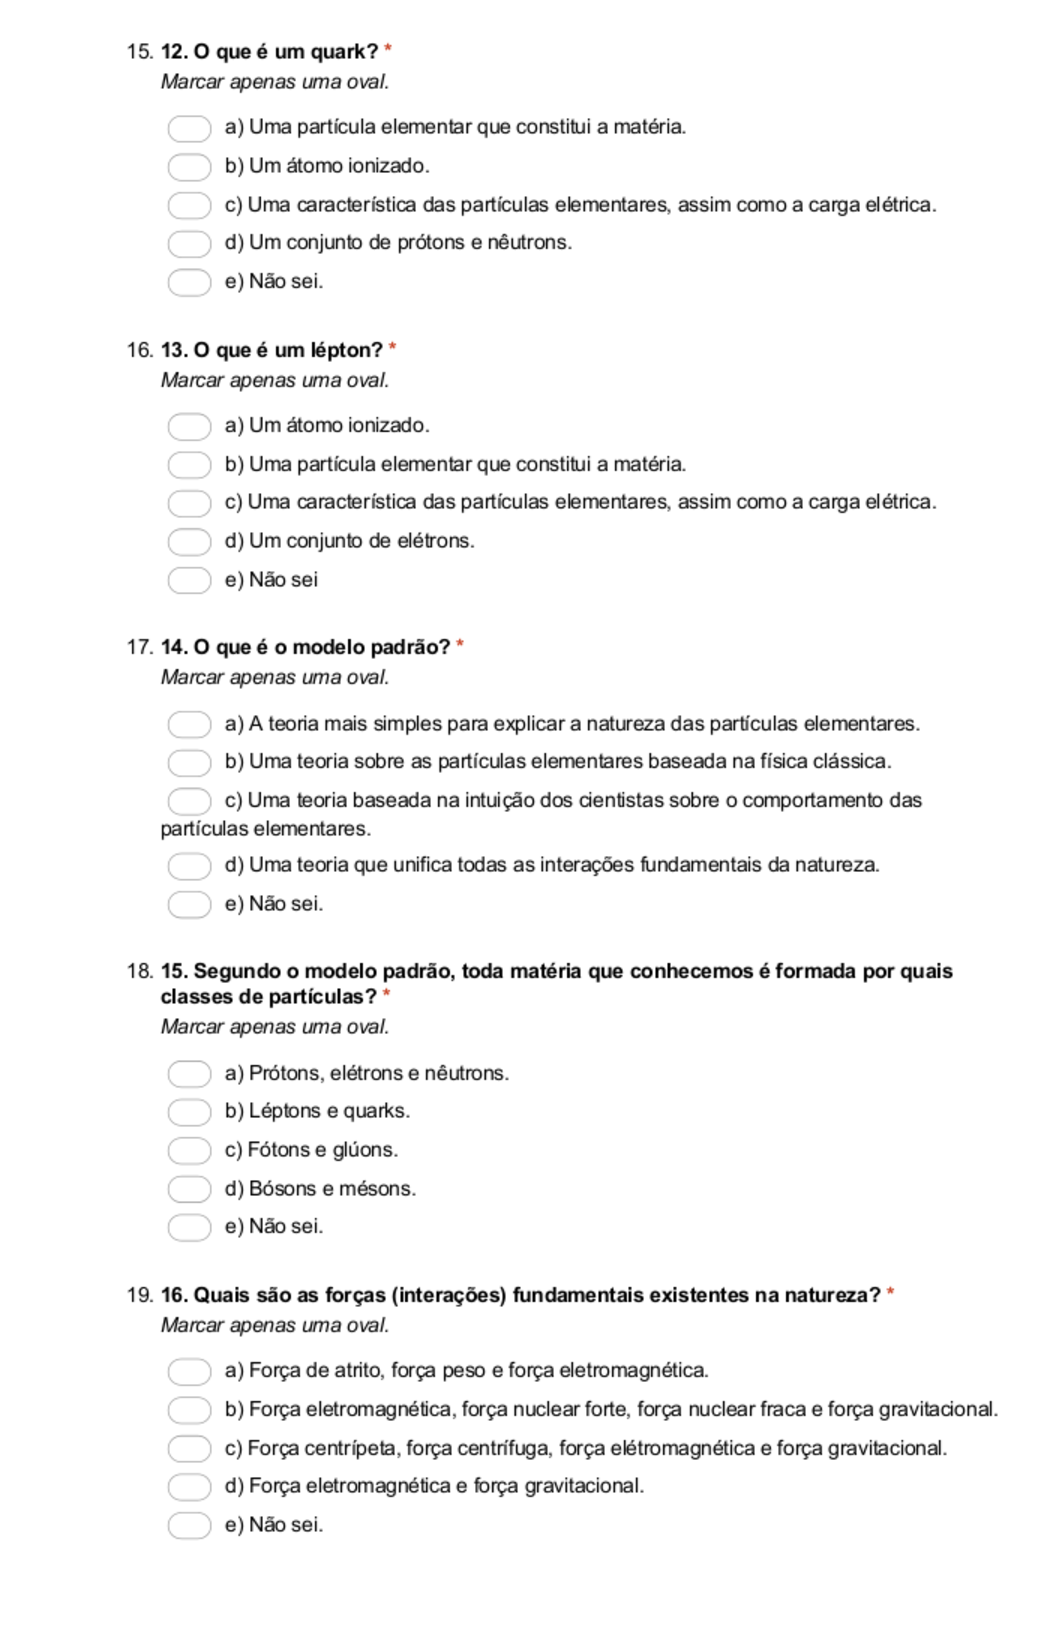
\includegraphics[width=0.70 \textwidth]{ApeB/Img_test/teste_part4}
	\caption{Teste: parte 4}
	\label{fig:pf_perg_16}
\end{figura}

\newpage

\begin{figura}[ht]
	\centering
	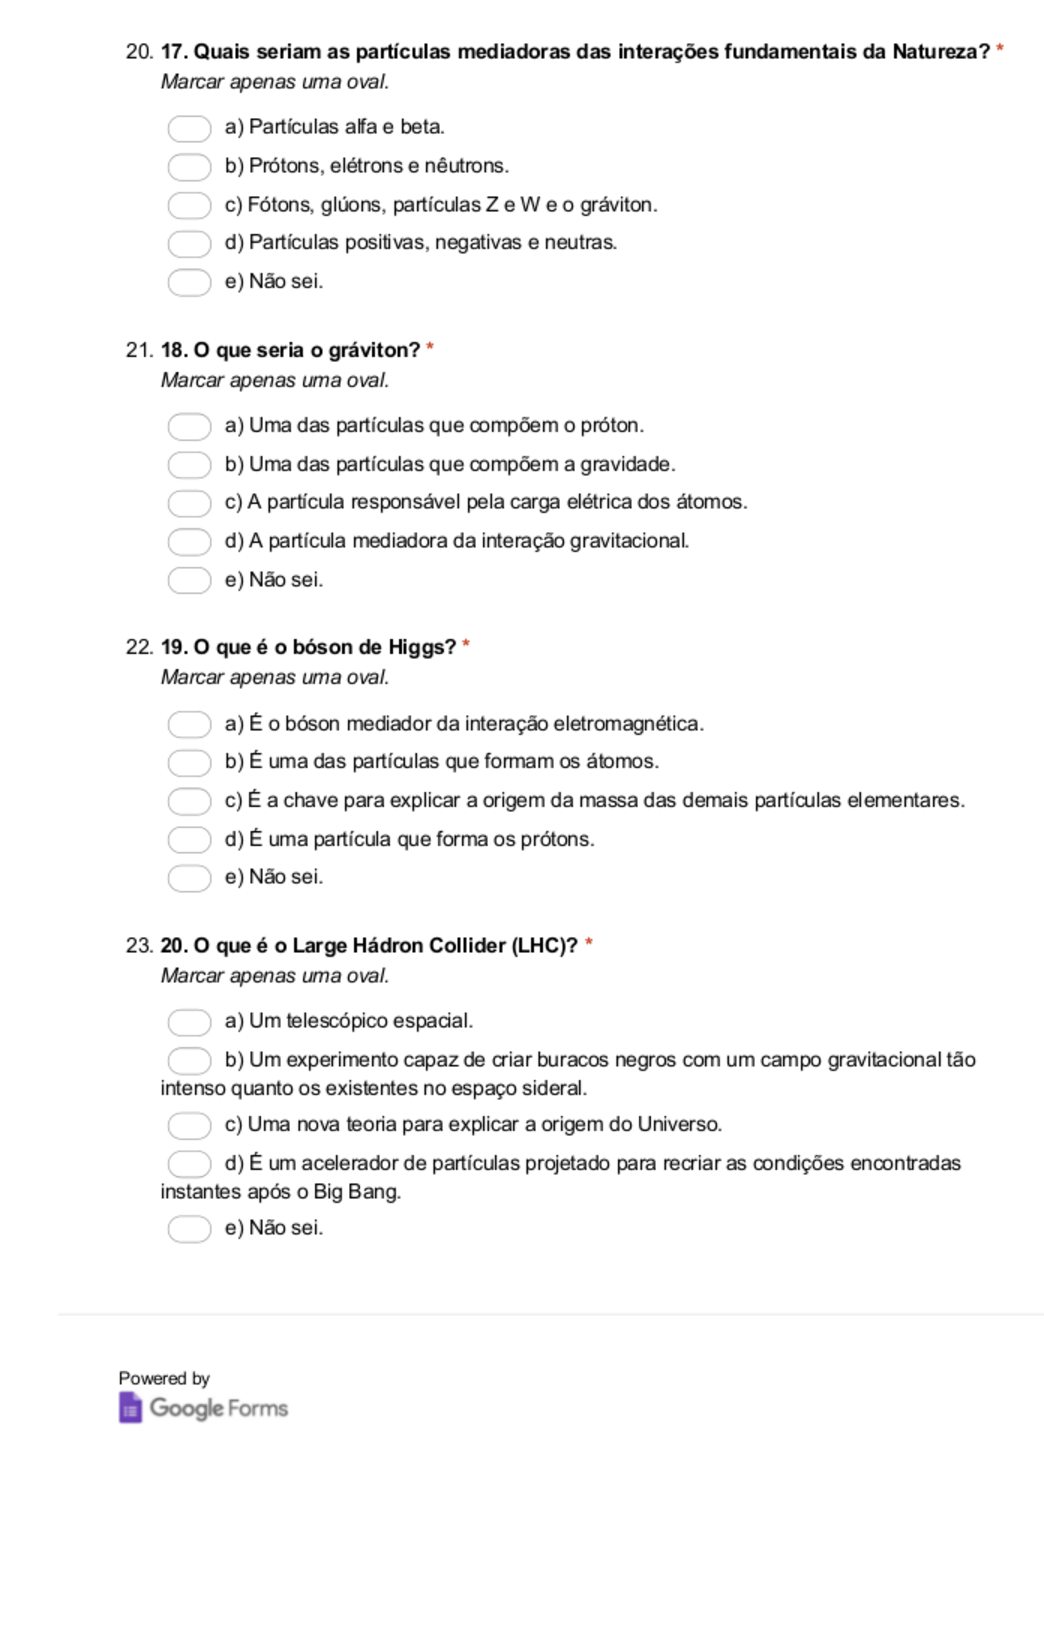
\includegraphics[width=0.70 \textwidth]{ApeB/Img_test/teste_part5}
	\caption{Teste: parte 5}
	\label{fig:pf_perg_16}
\end{figura}

\newpage

\section{Pesquisa Final}\label{app_b:final}

\begin{figura}[h]
	\centering
	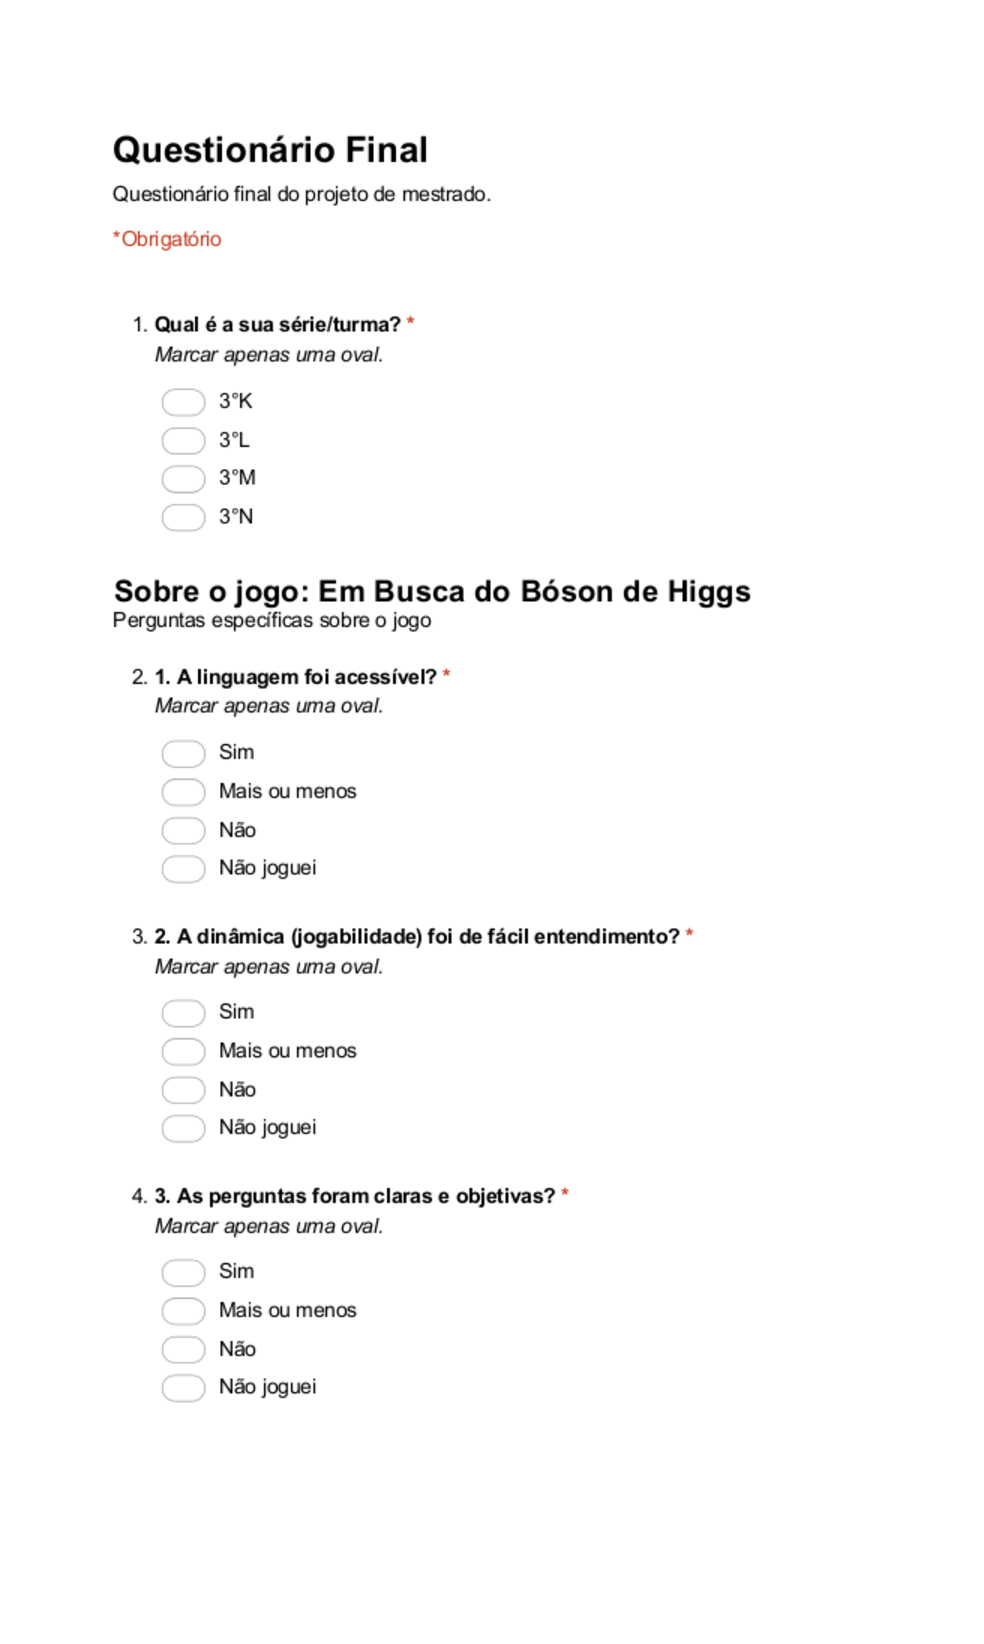
\includegraphics[width=0.69 \textwidth]{ApeB/Img_pesq_fin/pf_part1}
	\caption{Pesquisa final: parte 1}
	\label{fig:pf_perg_16}
\end{figura}

\begin{figura}[h]
	\centering
	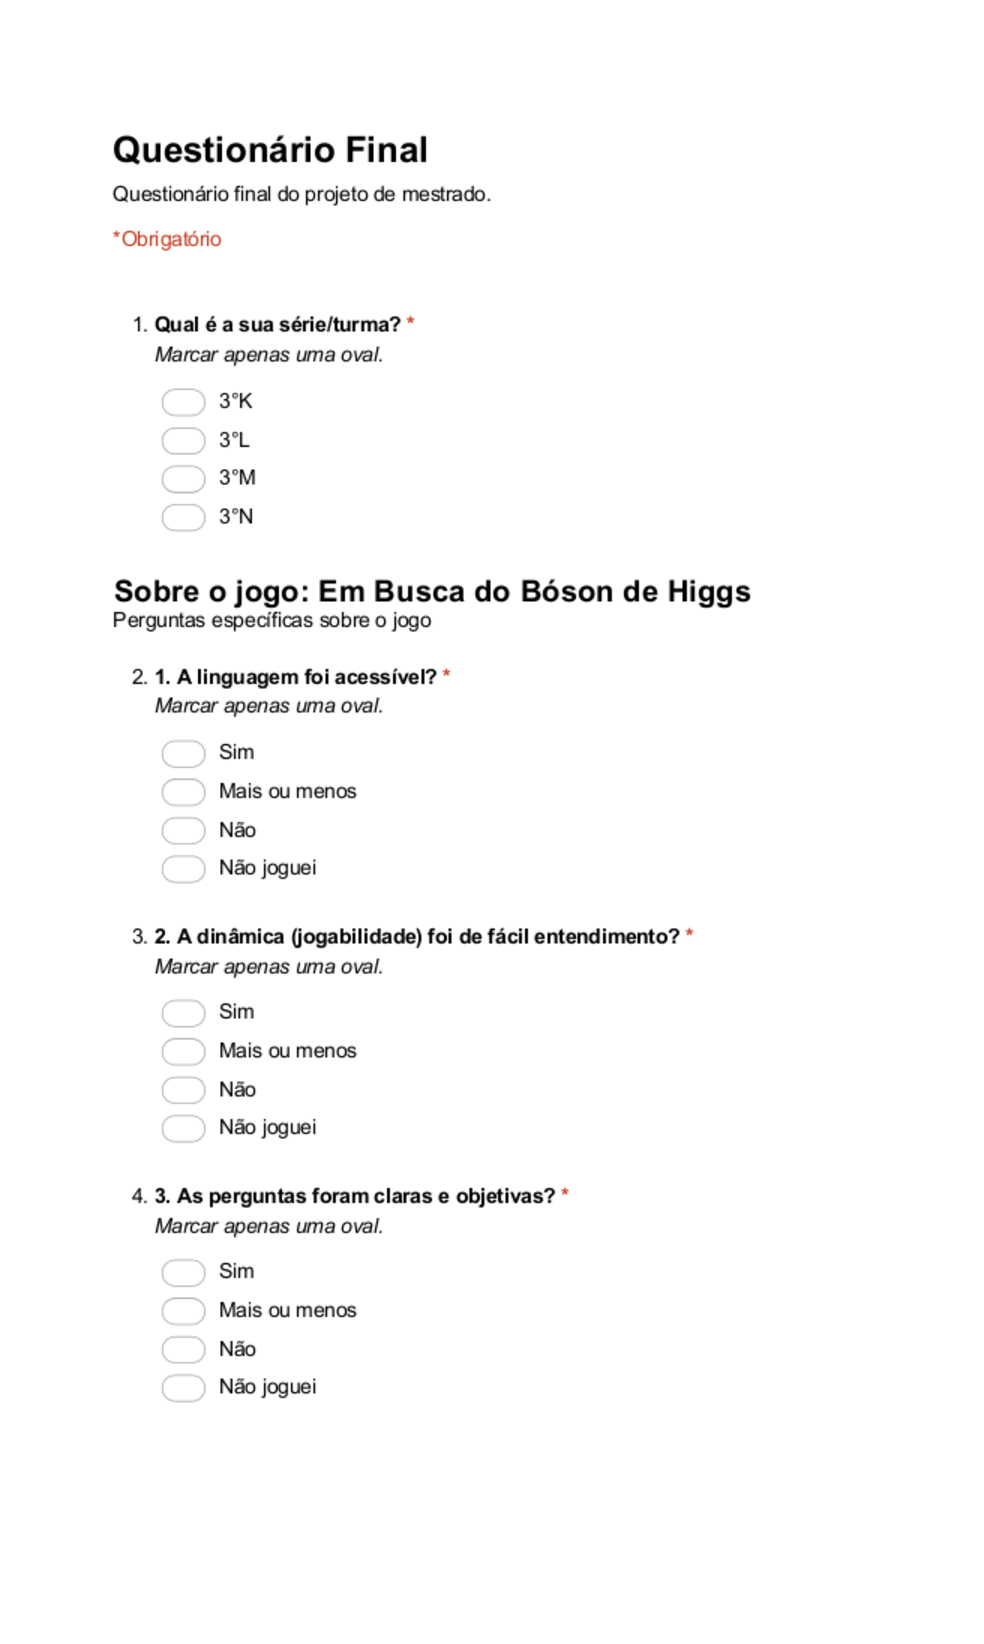
\includegraphics[width=0.69 \textwidth]{ApeB/Img_pesq_fin/pf_part1}
	\caption{Pesquisa final: parte 2}
	\label{fig:pf_perg_16}
\end{figura}

\begin{figura}[h]
	\centering
	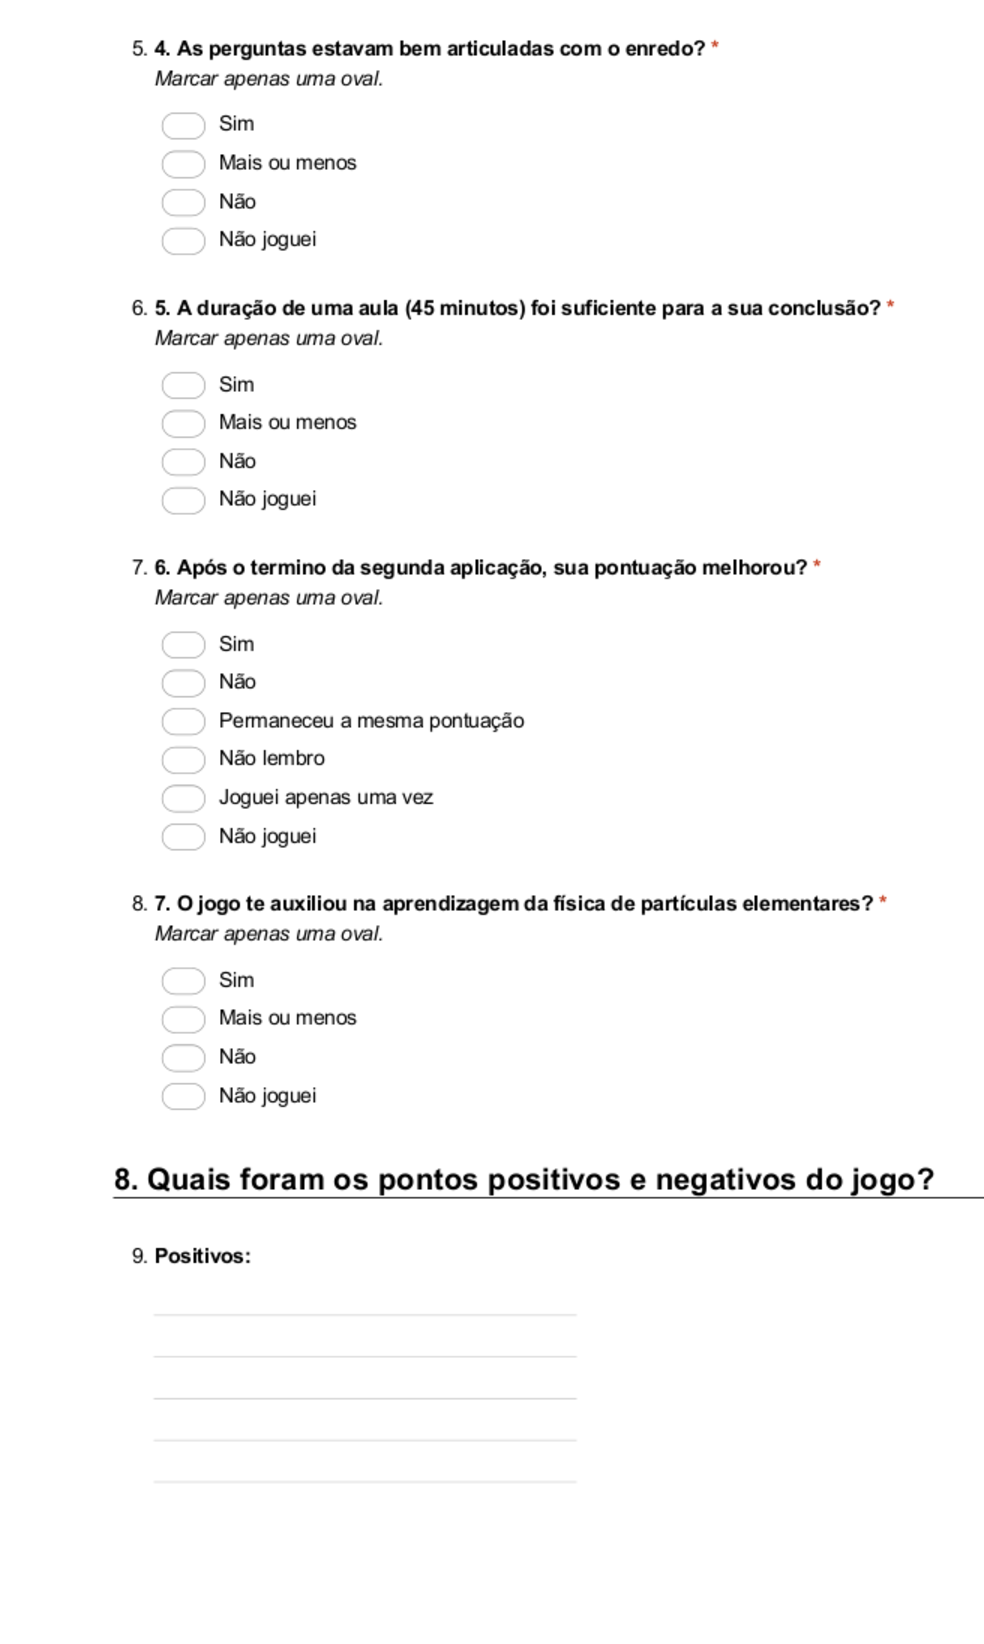
\includegraphics[width=0.69 \textwidth]{ApeB/Img_pesq_fin/pf_part2}
	\caption{Pesquisa final: parte 3}
	\label{fig:pf_perg_16}
\end{figura}

\begin{figura}[h]
	\centering
	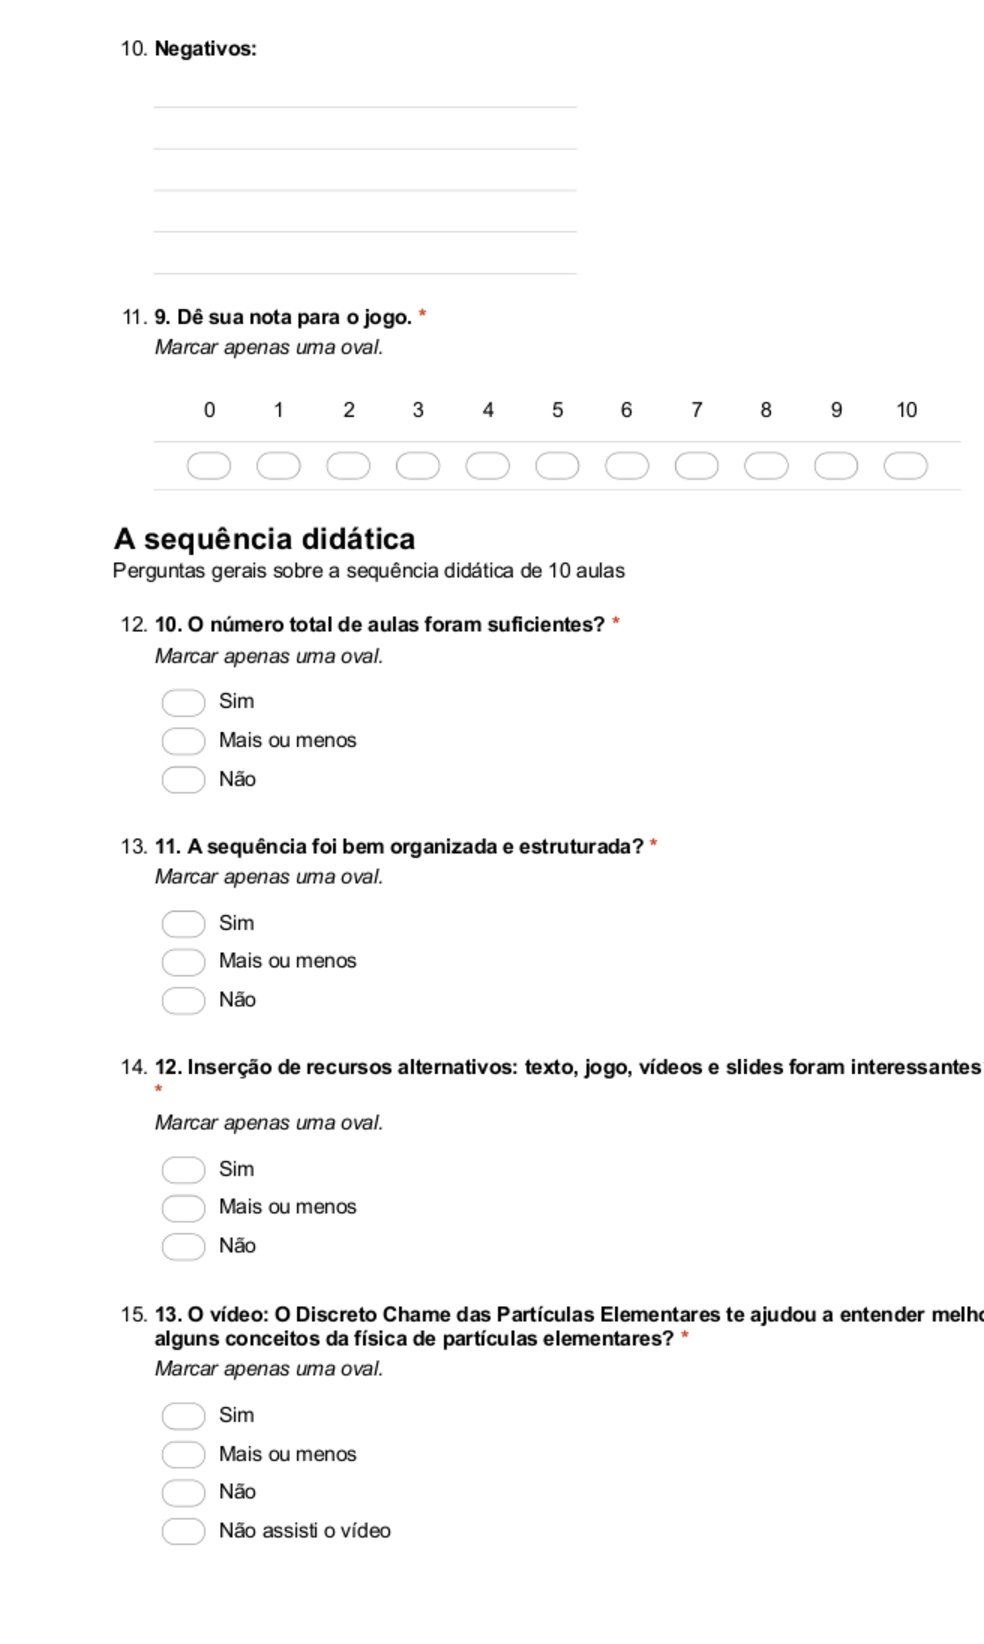
\includegraphics[width=0.69 \textwidth]{ApeB/Img_pesq_fin/pf_part3}
	\caption{Pesquisa final: parte 4}
	\label{fig:pf_perg_16}
\end{figura}

\begin{figura}[h]
	\centering
	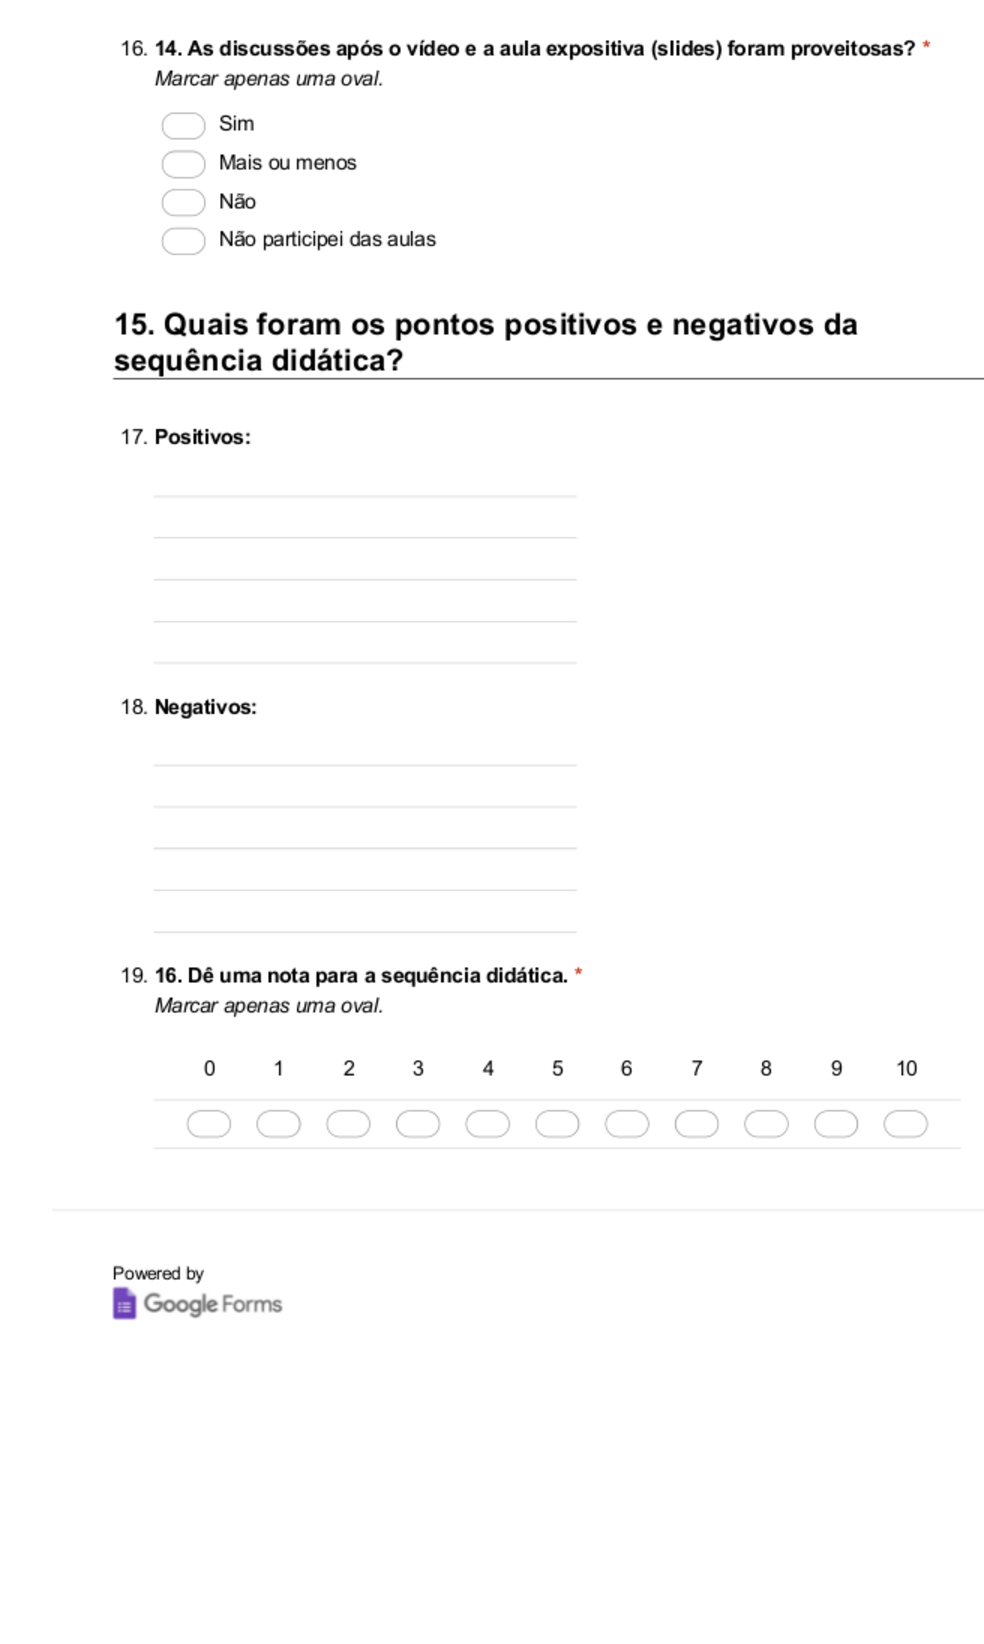
\includegraphics[width=0.69 \textwidth]{ApeB/Img_pesq_fin/pf_part4}
	\caption{Pesquisa final: parte 5}
	\label{fig:pf_perg_16}
\end{figura}

%\begin{figure}[h]
%\centering
%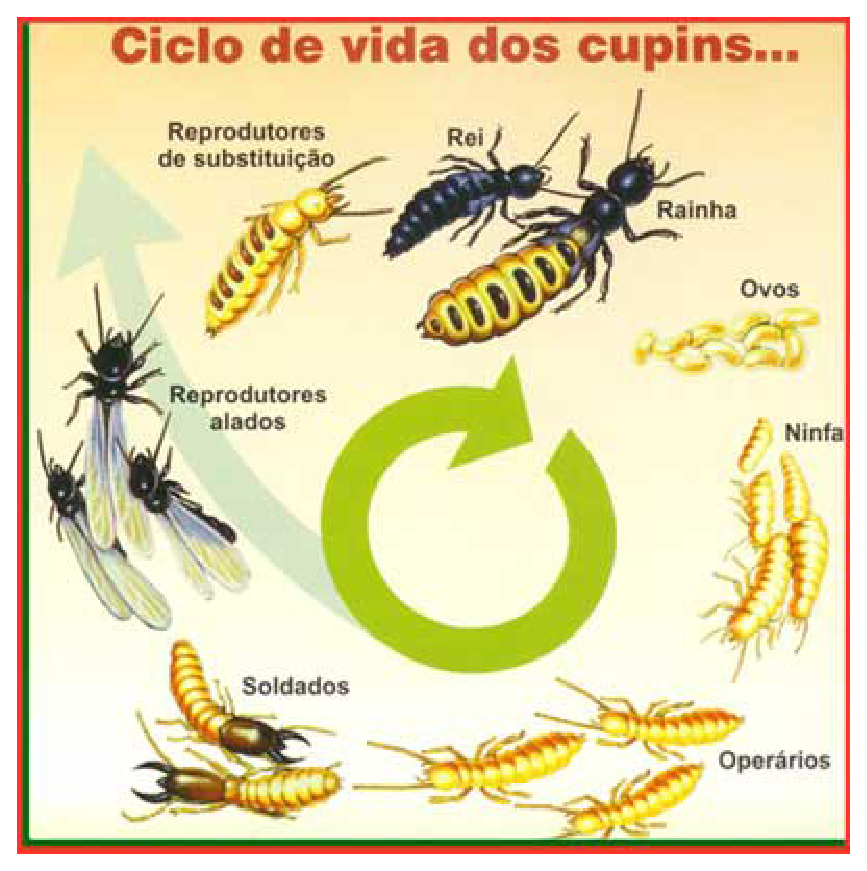
\includegraphics[height=5cm, width=5cm]{ApeA/pragas_ciclo_cupim}
%\caption{Uma figura que est� no ap�ndice}\label{FD}
%\end{figure}
